\documentclass[11pt]{article}

\usepackage[margin=1in]{geometry}
\usepackage[T1]{fontenc}
\usepackage[utf8]{inputenc}
\usepackage{amsmath,amssymb}
\usepackage{graphicx}
\usepackage{booktabs}
\usepackage{float}
\usepackage{url}
\usepackage{listings}
\usepackage{xcolor}

\lstset{
    basicstyle=\ttfamily\small,
    breaklines=true,
    frame=single,
    backgroundcolor=\color{gray!8},
    showstringspaces=false
}

\title{Comb Filters: Theory, Implementation, and MATLAB Demonstration}
\author{Group \#\underline{\hspace{2cm}} \\
\underline{\hspace{4cm}} \and \underline{\hspace{4cm}} \and \underline{\hspace{4cm}}}
\date{SEG800}

\begin{document}

\maketitle

\begin{abstract}
This tutorial introduces comb filters, a class of digital filters formed by combining a signal with a delayed version of itself. It explains the difference between feedforward and feedback comb filters, presents their basic system functions, and shows why their frequency responses contain evenly spaced peaks or notches. A MATLAB demonstration using a simple two-tone input signal is included to connect the theory with a practical example. The results show that the delay controls the spacing of the comb teeth, while the gain controls the strength of the filtering effect. These properties make comb filters useful in audio processing tasks such as echo, reverberation, harmonic enhancement, and periodic interference removal.
\end{abstract}

\section{Introduction}
Comb filters are an important topic in digital signal processing because they provide a simple way to shape the frequency content of a signal using delay. Their name comes from the appearance of the frequency response, which resembles the teeth of a comb. Depending on the filter structure, some frequencies are reinforced while others are reduced or completely cancelled.

The key idea behind a comb filter is interference. When a signal is added to a delayed copy of itself, some frequency components line up in phase and become stronger, while others do not line up and become weaker. Because this pattern repeats regularly across the frequency axis, the response contains equally spaced peaks or equally spaced notches.

Comb filters are widely used in audio and speech processing. Common applications include echo and delay effects, reverberation design, periodic noise removal, and harmonic shaping. They are also a strong educational example because the mathematics is manageable and the time-domain behavior is easy to demonstrate in MATLAB.

\section{Theory of Comb Filters}
\subsection{Basic Idea}
In discrete-time signal processing, a delay of $D$ samples shifts a signal by $D$ positions in time. If the original signal is denoted by $x[n]$, then the delayed version is $x[n-D]$. A comb filter uses this delayed signal in either a feedforward or a feedback structure.

The delay introduces a phase shift that depends on frequency. Because different frequencies experience different phase relationships between the original and delayed signals, some are amplified and some are attenuated. This alternating pattern creates the comb-like frequency response.

\subsection{Feedforward Comb Filter}
The feedforward comb filter is defined by the difference equation
\begin{equation}
    y[n] = x[n] + a x[n-D]
\end{equation}
where $x[n]$ is the input signal, $y[n]$ is the output signal, $D$ is the delay in samples, and $a$ is the gain applied to the delayed term.

Taking the $z$-transform of the difference equation gives the system function
\begin{equation}
    H_{\mathrm{ff}}(z) = \frac{Y(z)}{X(z)} = 1 + a z^{-D}
\end{equation}

This expression shows that the filter is simple to implement because it only requires the present input sample and one delayed input sample. When $a = 1$, the filter creates exact notches at frequencies where the delayed signal is out of phase with the original signal.

\subsection{Feedback Comb Filter}
The feedback comb filter is defined by
\begin{equation}
    y[n] = x[n] + a y[n-D]
\end{equation}

Rearranging and taking the $z$-transform gives
\begin{equation}
    H_{\mathrm{fb}}(z) = \frac{Y(z)}{X(z)} = \frac{1}{1 - a z^{-D}}
\end{equation}

Unlike the feedforward structure, the feedback comb filter feeds previous output samples back into the system. As a result, it produces stronger resonant peaks. For a stable causal feedback comb filter, the gain is typically chosen so that $|a| < 1$.

\subsection{Comb Tooth Spacing}
One of the most important properties of a comb filter is the spacing between adjacent teeth in the frequency response. If the sampling frequency is $F_s$, then the spacing is approximately
\begin{equation}
    \Delta f = \frac{F_s}{D}
    \label{eq:comb_spacing}
\end{equation}

This means that increasing the delay produces teeth that are closer together, while decreasing the delay produces teeth that are farther apart. In the MATLAB demonstration used in this tutorial,
\begin{equation}
    \Delta f = \frac{8000}{40} = 200\ \text{Hz}
\end{equation}

Therefore, the frequency response repeats every 200 Hz.

\section{Frequency-Domain Interpretation}
The comb pattern can be understood by studying the phase relationship between a signal and its delayed copy. For some frequencies, the delayed component adds constructively to the original signal. At those frequencies, the magnitude response is large. For other frequencies, the delayed component adds destructively, causing attenuation or cancellation.

For the feedforward case with $a = 1$, the first notch occurs at
\begin{equation}
    f_{\mathrm{notch},1} = \frac{F_s}{2D}
\end{equation}

Using the parameters in this project,
\begin{equation}
    f_{\mathrm{notch},1} = \frac{8000}{2 \cdot 40} = 100\ \text{Hz}
\end{equation}

Since the notch pattern repeats every 200 Hz, other notches occur near 300 Hz, 500 Hz, 700 Hz, and so on. This is why the 300 Hz tone in the MATLAB demonstration is strongly attenuated by the feedforward comb filter.

In the feedback case, the same spacing appears, but the structure emphasizes resonances instead of exact cancellations. The result is a response with narrow, repeated peaks.

\section{MATLAB Implementation}
The MATLAB file used in this assignment is \texttt{comb\_filter\_demo.m}. The script is written as a single, top-down file so that it is easy to read, maintain, and explain to classmates. The overall workflow of the script is:

\begin{enumerate}
    \item Define the sampling rate, delay, gains, and signal duration.
    \item Create a test signal containing two sinusoidal components.
    \item Build the feedforward comb filter coefficients.
    \item Build the feedback comb filter coefficients.
    \item Filter the input signal and plot the outputs.
    \item Plot the frequency responses and spectrum comparisons.
\end{enumerate}

The script uses a synthetic two-tone input signal because this makes the comb filtering effect easy to see. The 300 Hz component is chosen near a feedforward notch, while the 400 Hz component lies between notches and remains stronger.

The coefficient construction is simple. For the feedforward filter, the numerator contains two nonzero values: one at the current sample and one at the delayed position. For the feedback filter, the denominator contains the delayed feedback term. A simplified version of the idea is shown below.

\begin{lstlisting}[language=Matlab, caption={Simplified coefficient construction for the comb filters.}]
% Feedforward comb filter
numerator = zeros(1, delaySamples + 1);
numerator(1) = 1;
numerator(end) = feedforwardGain;
denominator = 1;

% Feedback comb filter
numerator = 1;
denominator = zeros(1, delaySamples + 1);
denominator(1) = 1;
denominator(end) = -feedbackGain;
\end{lstlisting}

The MATLAB \texttt{filter} function is then used to apply each filter to the input signal. The script also plots the time-domain output, the frequency response, and the output spectrum so that the theoretical discussion can be compared with the numerical results.

\section{Experimental Setup}
Table~\ref{tab:parameters} summarizes the parameters used in the MATLAB demonstration.

\begin{table}[H]
    \centering
    \caption{Parameters used in the comb filter demonstration.}
    \label{tab:parameters}
    \begin{tabular}{ll}
        \toprule
        Parameter & Value \\
        \midrule
        Sampling frequency $F_s$ & 8000 Hz \\
        Signal duration & 0.05 s \\
        Delay $D$ & 40 samples \\
        Feedforward gain & 1.0 \\
        Feedback gain & 0.7 \\
        Input tone 1 & 300 Hz \\
        Input tone 2 & 400 Hz \\
        Comb spacing $\Delta f$ & 200 Hz \\
        \bottomrule
    \end{tabular}
\end{table}

The choice of 300 Hz and 400 Hz is intentional. Because the feedforward comb filter has notches repeating every 200 Hz, the 300 Hz tone lies close to one of the notches, while the 400 Hz tone lies between notches. This makes the spectrum comparison easy to interpret.

\section{Results and Discussion}
\subsection{Input Signal}
Figure~\ref{fig:input_signal} shows the input signal created from the sum of two sinusoids. The waveform is more complex than a single tone because it contains both 300 Hz and 400 Hz components.

\begin{figure}[H]
    \centering
    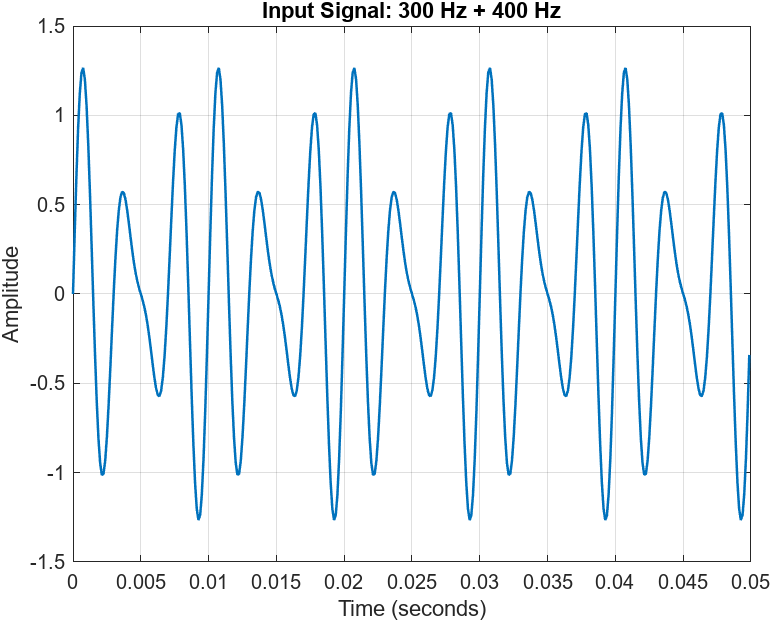
\includegraphics[width=0.9\textwidth]{artifacts/fig1.png}
    \caption{Input signal used in the MATLAB demonstration.}
    \label{fig:input_signal}
\end{figure}

\subsection{Time-Domain Output Comparison}
Figure~\ref{fig:time_domain} compares the input, the feedforward output, and the feedback output over the first 20 ms. The feedforward output remains bounded and periodic, while the feedback output shows a stronger resonant shape because past output samples continue to influence the current response.

\begin{figure}[H]
    \centering
    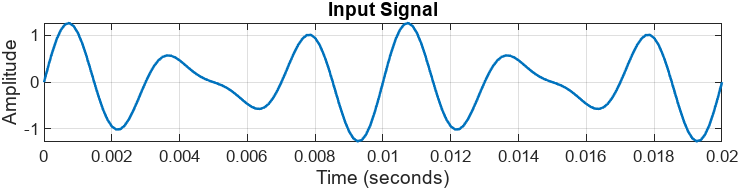
\includegraphics[width=0.9\textwidth]{artifacts/fig2.png}
    \caption{Time-domain comparison of the input, feedforward output, and feedback output.}
    \label{fig:time_domain}
\end{figure}

\subsection{Frequency Response}
Figure~\ref{fig:frequency_response} shows the most important result in the tutorial. The feedforward comb filter has repeated notches and peaks across the frequency axis. The feedback comb filter shows repeated narrow resonances. In both cases, the spacing between adjacent teeth is approximately 200 Hz, which matches the theoretical value from Equation~\eqref{eq:comb_spacing}.

\begin{figure}[H]
    \centering
    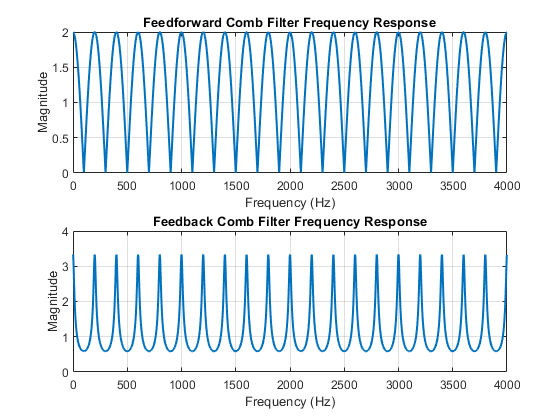
\includegraphics[width=0.9\textwidth]{artifacts/fig3.png}
    \caption{Frequency responses of the feedforward and feedback comb filters.}
    \label{fig:frequency_response}
\end{figure}

\subsection{Feedforward Spectrum Comparison}
Figure~\ref{fig:feedforward_spectrum} compares the input spectrum with the feedforward output spectrum. The 300 Hz component is strongly reduced because it falls close to a notch frequency, while the 400 Hz component remains more prominent. This confirms the expected notch behavior of the feedforward comb filter.

\begin{figure}[H]
    \centering
    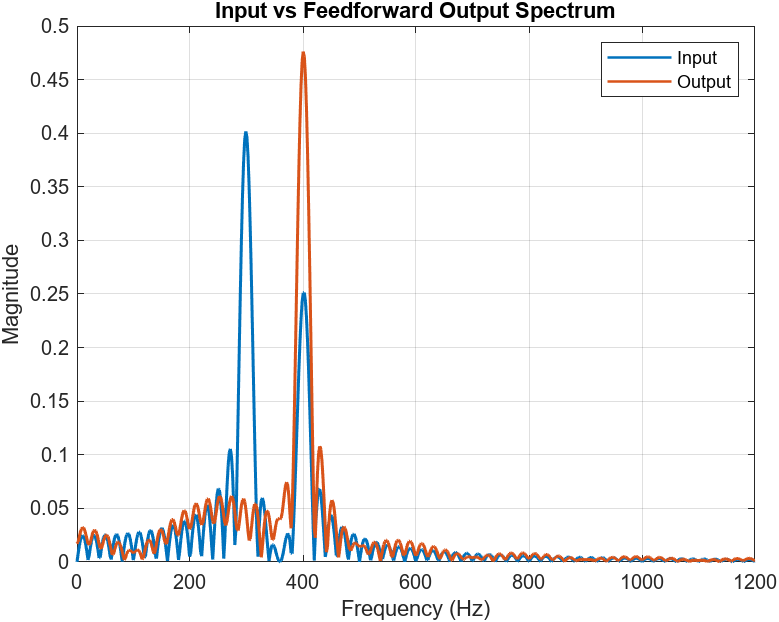
\includegraphics[width=0.9\textwidth]{artifacts/fig4.png}
    \caption{Spectrum comparison between the input signal and the feedforward comb filter output.}
    \label{fig:feedforward_spectrum}
\end{figure}

\subsection{Feedback Spectrum Comparison}
Figure~\ref{fig:feedback_spectrum} compares the input spectrum with the feedback output spectrum. In this case, the filter produces stronger resonant behavior, especially near the repeated peak frequencies. This demonstrates that the feedback structure emphasizes selected frequencies more aggressively than the feedforward structure.

\begin{figure}[H]
    \centering
    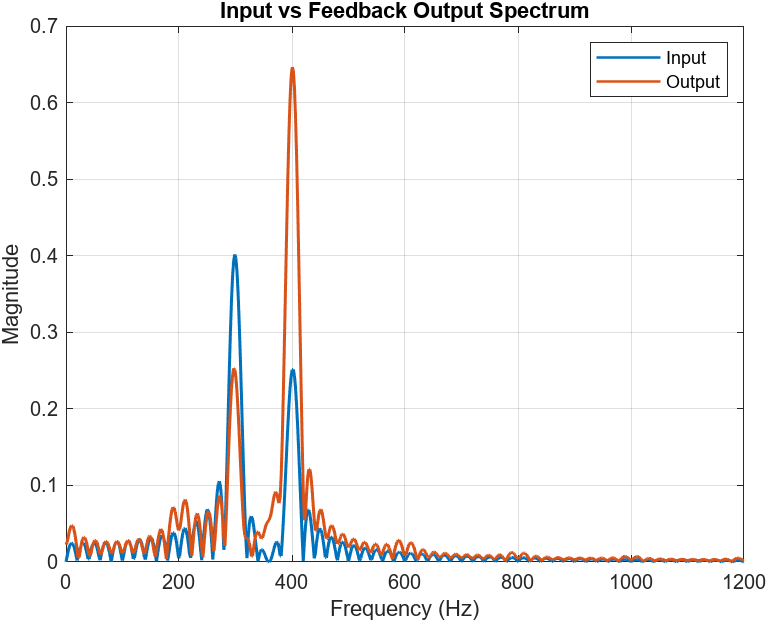
\includegraphics[width=0.9\textwidth]{artifacts/fig5.png}
    \caption{Spectrum comparison between the input signal and the feedback comb filter output.}
    \label{fig:feedback_spectrum}
\end{figure}

Overall, the MATLAB results agree with the theoretical discussion. The delay controls the spacing between comb teeth, and the gain controls how strong the effect becomes. The feedforward filter is useful for repeated notching, while the feedback filter is more suitable for repeated resonance.

\section{Applications of Comb Filters}
Comb filters are useful in several practical DSP applications:

\begin{itemize}
    \item \textbf{Echo and delay effects:} A delayed version of the signal can be added back to create an audible echo.
    \item \textbf{Reverberation design:} Feedback comb filters are common building blocks in artificial reverberation systems.
    \item \textbf{Periodic interference removal:} Repeated notches can suppress harmonically related unwanted components.
    \item \textbf{Harmonic enhancement:} Repeated resonances can emphasize harmonic content in audio signals.
    \item \textbf{Speech and music processing:} Comb filters are used in tone shaping, special effects, and acoustic modeling.
\end{itemize}

These applications are one reason comb filters remain a standard example in DSP education and practice.

\section{Conclusion}
This tutorial explained the theory and implementation of comb filters using both feedforward and feedback structures. A comb filter works by combining a signal with a delayed version of itself, which creates repeated constructive and destructive interference across the frequency axis. The feedforward comb filter creates repeated notches and peaks, while the feedback comb filter creates repeated resonant peaks.

The MATLAB demonstration confirmed the theory. With a sampling frequency of 8000 Hz and a delay of 40 samples, the spacing between comb teeth was 200 Hz. The feedforward filter attenuated the 300 Hz input tone because it lay near a notch, while the feedback filter emphasized repeated resonant frequencies.

Comb filters are simple to implement, easy to visualize, and useful in many real-world signal processing applications. For these reasons, they are a strong topic for both classroom learning and practical DSP work.

\begin{thebibliography}{9}

\bibitem{proakis}
J. G. Proakis and D. G. Manolakis,
\textit{Digital Signal Processing: Principles, Algorithms, and Applications},
4th ed., Pearson, 2007.

\bibitem{mathworks-filter}
MathWorks,
``filter,''
\url{https://www.mathworks.com/help/matlab/ref/filter.html}

\bibitem{mathworks-freqz}
MathWorks,
``freqz,''
\url{https://www.mathworks.com/help/signal/ref/freqz.html}

\end{thebibliography}

\end{document}
